\documentclass[11pt]{article}

% --- Page geometry & fonts ----------------------------------------------
\usepackage[margin=1in]{geometry}
\usepackage[T1]{fontenc}
\usepackage{lmodern}
\usepackage[default,osfigures]{opensans}
\renewcommand{\familydefault}{\sfdefault}
\usepackage{microtype}

% --- Color palette ------------------------------------------------------
\usepackage{xcolor}
\definecolor{accent}{HTML}{1F4E79}
\definecolor{accentLight}{HTML}{2E75B6}
\definecolor{rule}{HTML}{B7C7D6}
\definecolor{soft}{HTML}{F4F7FB}
\definecolor{ink}{HTML}{1A1A1A}
\definecolor{muted}{HTML}{555555}

% --- Layout / typography ------------------------------------------------
\usepackage[hidelinks]{hyperref}
\hypersetup{colorlinks=true, linkcolor=accent, urlcolor=accent}
\usepackage{enumitem}
\usepackage{graphicx}
\usepackage{titlesec}
\usepackage{titling}
\usepackage{parskip}
\usepackage{fancyhdr}
\usepackage{caption}
\usepackage{tcolorbox}
\tcbuselibrary{skins}

\captionsetup{font={small,it,color=muted}, labelformat=empty, skip=4pt}
\setlist{itemsep=3pt, topsep=3pt, parsep=0pt, leftmargin=1.3em}
\color{ink}

\titleformat{\section}
  {\color{accent}\Large\bfseries}
  {}{0pt}
  {}
  [\vspace{2pt}{\color{rule}\titlerule[0.6pt]}]
\titlespacing*{\section}{0pt}{1.6em}{0.7em}

\titleformat{\subsection}
  {\color{accentLight}\normalsize\bfseries}{}{0pt}{}
\titlespacing*{\subsection}{0pt}{1.0em}{0.3em}

\pagestyle{fancy}
\fancyhf{}
\renewcommand{\headrulewidth}{0pt}
\fancyfoot[C]{\small\color{muted}\thepage}

\pretitle{\begin{flushleft}\color{accent}\Huge\bfseries}
\posttitle{\par\vspace{2pt}{\color{rule}\rule{\linewidth}{0.8pt}}\end{flushleft}\vspace{-0.4em}}
\preauthor{}\postauthor{}
\predate{\begin{flushleft}\color{muted}\small}
\postdate{\end{flushleft}}

\title{Data-Cleaning Benchmark Generator\,---\,Progress Update}
\author{}
\date{\today}

\newtcolorbox{callout}{
  enhanced, breakable,
  colback=soft, colframe=rule,
  boxrule=0.4pt, arc=2pt,
  left=10pt, right=10pt, top=6pt, bottom=6pt,
  before skip=6pt, after skip=8pt,
}

\begin{document}
\maketitle
\vspace{-0.6em}

\section*{Project overview}
Dirty data remains one of the most expensive problems in
analytics: surveys consistently report that data scientists
spend the majority of their time --- around 80\% in widely
cited industry reports such as Gartner and Anaconda --- on
data preparation rather than analysis. To measure progress on
automated data-cleaning systems, the research community relies
on a small set of established benchmarks (e.g.\ Hospital,
Beers, Flights, Rayyan, Tax), most of which are either
hand-curated at modest scale or constructed by injecting
synthetic errors into otherwise clean tables. Recent
evaluation studies (e.g.\ Mahdavi et al.\ on \emph{Raha},
Abdelaal et al.\ on \emph{REIN}) have noted that these
benchmarks under-represent the diversity of real-world errors
and that no widely adopted methodology exists for quantifying
how complete a benchmark actually is.

We are building a system intended to address both gaps. It
constructs data-cleaning benchmarks directly from real
spreadsheet and CSV files using a \emph{human-in-the-loop}
design: an LLM scans each table and surfaces a focused queue
of likely-error cells, and a human reviewer remains the final
authority and signs off every entry through a dedicated web
UI. On top of this, a statistical layer attaches a
\emph{completeness guarantee} to the LLM stage --- a
quantified estimate of how many real errors the LLM is
likely to have missed. That estimate serves two purposes.
The system uses it internally to decide where to spend
additional LLM scans, focusing on the parts of the data that
still look incomplete and skipping the parts that already
look saturated. The same signal is shown to the reviewer in
the labelling UI, so labelling effort can be directed by
statistical need rather than walking the queue uniformly.
The deliverable is a labelled benchmark of real-world errors
in which every confirmed entry has been signed off by a
human, and every region of the dataset carries an explicit
estimate of how complete it is --- a property existing
public benchmarks do not provide.

The rest of this update first fixes the set of error types the
benchmark targets, then describes each component of the system
in turn, reports current implementation status, and outlines
the planned validation experiment.

% ------------------------------------------------------------------------
\section*{Scope: error taxonomy}
This section fixes the set of error categories the system is
designed to detect; subsequent sections describe the components
that operate on this taxonomy. The benchmark covers nine error
categories, grouped by the structural scope at which the error
manifests. A representative example is given for each.

\subsection*{Within a single column (4)}
\begin{itemize}
  \item \textbf{Typo} --- ``Unietd States'' vs.\ ``United States''.
  \item \textbf{Single-column inconsistency} --- ``USA'' vs.\
    ``U.S.A.''; ``james smith'' vs.\ ``James Smith'';
    ``10,000'' vs.\ ``10000''; ``15\%'' mixed with ``0.15''
    in one column.
  \item \textbf{Semantically incompatible value} --- a phone
    number sitting in a ``Name'' column.
  \item \textbf{Numeric outlier} --- a \$1,000,000 salary in a
    column whose values otherwise sit between \$40k and \$120k.
\end{itemize}

\subsection*{Within a row, across columns (3)}
\begin{itemize}
  \item \textbf{Functional-dependency violation} --- ZIP
    ``10001'' paired with State ``California''.
  \item \textbf{Numeric calculation inconsistency} ---
    Qty $3 \times$ Price \$10 with Total \$25.
  \item \textbf{String calculation inconsistency} --- First
    ``Jane'', Last ``Doe'', Full Name ``John Doe''.
\end{itemize}

\subsection*{Across rows (1)}
\begin{itemize}
  \item \textbf{Row duplication} --- the same transaction
    recorded twice.
\end{itemize}

\subsection*{Across tables (1)}
\begin{itemize}
  \item \textbf{Inter-table inconsistency} --- the same entity's
    name differs across tables (e.g.\ ``Acme Corp.'' in the
    Customers table vs.\ ``ACME Corporation'' in the Orders
    table).
\end{itemize}

% ------------------------------------------------------------------------
\section*{Construction pipeline}
The construction pipeline is the first system component: it
transforms a raw table into a queue of candidate errors for
human review. A run processes a CSV, spreadsheet, or folder
through the stages below, in the order listed. Stage~1
recovers the table's multi-column structure --- functional
dependencies, arithmetic identities, and string-composition
rules --- and emits the rows that already violate it. Stage~2
then runs the per-type cell-level scans with those rules and
their violating rows attached to the prompt, so that the
LLM does not have to rediscover ``Total = Qty\,$\times$\,Price''
on every chunk and can spend its budget on the single-column
issues and on cells the structural layer cannot already
explain.

\begin{enumerate}
  \item \textbf{Relation discovery (multi-column rules).}
    The LLM proposes candidate structural rules from a
    compact per-table digest (e.g.\
    ``Total = Quantity $\times$ Price'',
    ``ZIP determines State'',
    ``Full Name = First + ` ' + Last''), and pre-verifies
    each rule by emitting a small \texttt{check(df)} Python
    function that is executed in a sandbox over the table.
    Rules that pass become structural priors for stage~2;
    their violating rows are persisted as high-confidence
    candidates.

  \item \textbf{Per-type LLM scan.} Tables are chunked,
    and for each error type the LLM is queried with one
    focused prompt over the chunk together with a compact
    table digest (column types, sample values, simple
    statistics). Stage~1 contributes its own
    rule-violating rows directly into the candidate queue,
    where they are merged with the per-type findings in
    stage~3; threading the discovered rules into the
    per-type prompt itself as explicit priors is the
    immediate next integration step.

  \item \textbf{Grouping and explanation.} Findings from the
    relation and per-type stages that overlap on the same
    cell are merged deterministically into a single
    candidate. An optional LLM synthesis pass produces a
    canonical explanation, suggested fix, and confidence
    score for multi-type clusters, and flags low-confidence
    cases.

  \item \textbf{Web verification.} For candidates whose
    value is a real-world named entity (organisation,
    address, phone, URL), a web search is issued and the
    LLM produces a verdict (\emph{confirmed error},
    \emph{false positive}, \emph{ambiguous}) using only
    the retrieved snippets. The verdict either attaches a
    citation to the candidate or removes it from the queue.

  \item \textbf{Human review.} Every candidate produced by
    the pipeline is presented to a human reviewer in the
    labelling UI for labelling. Confirmed candidates form
    the benchmark; rejected candidates are retained as
    hard negatives.
\end{enumerate}

\begin{callout}
The pipeline alone returns a candidate queue but does not yet
quantify what it has missed. The next section describes the
statistical layer responsible for this completeness estimate.
\end{callout}

% ------------------------------------------------------------------------
\section*{Coverage estimator}
The coverage estimator is the second system component. It
answers a simple question: of all the real errors of a given
type sitting somewhere in this data, roughly how many is the
LLM still likely to be missing? It does so by treating each
slice of the data --- the whole dataset, a single column,
a column pair, a row, a CSV, a workbook, or a cross-table
relation --- as its own independent problem, paired with each
error type, and tracking it on its own. Each (slice,
error-type) pair is called an \emph{arm}. Arms are kept
separate rather than pooled so that one easy slice does not
mask another that is still incomplete.

To produce the signal the estimator needs, the LLM is run
over the same data several times under small, controlled
variations: a different row and column ordering on each pass,
and on later passes a re-worded version of the prompt. The
original row identifiers are preserved across passes so the
detections can be matched up. Across these passes, every
distinct candidate (keyed by its location and what the LLM
said about it) is tracked --- specifically, how many of the
passes it showed up in. Errors the LLM consistently fails
to find appear in this picture as candidates that the data
suggests \emph{should} be there but never get reported, and
estimating that hidden mass is the job of this component.

\begin{itemize}
  \item \textbf{What the estimator computes.} For each
    arm, the estimator looks at how often each candidate
    has been re-detected across passes. The intuition is
    standard in ecology and language modelling: if many
    candidates have been seen only once, the LLM is
    probably still finding new ones, so a lot is likely
    still missing; if almost every recent detection
    duplicates something already found, the well is
    running dry. From this frequency pattern the system
    derives three numbers per arm: the probability that
    the next scan will turn up a previously unseen
    candidate, an estimate of how many candidates remain
    unseen, and a false-negative rate (the estimated
    fraction of all real errors the LLM has so far
    missed). The underlying machinery is the
    Good--Turing / Chao1 family of estimators, which has
    a long track record on exactly this kind of
    rare-event extrapolation.
  \item \textbf{Adaptive loop and stop rule.} After every
    pass each arm is re-evaluated. An arm is marked
    \emph{saturated} when two conditions hold together:
    new candidates have stopped appearing at a meaningful
    rate, and the estimated missing fraction has dropped
    below the target tolerance (default 5\%). Both
    conditions must hold for two consecutive passes, and
    only after a minimum number of passes per arm.
    Saturated arms (and, once every arm of an error type
    saturates, the error type itself) are pruned from
    later LLM scans, so probe budget moves to the parts of
    the data still above target. Arms that hit the per-arm
    pass cap without saturating are marked
    \emph{exhausted} and flagged for follow-up.
  \item \textbf{Reviewer-facing signal.} The same per-arm
    status is exposed in the labelling UI alongside each
    candidate. Saturated arms are de-prioritised; arms
    still above target are surfaced as needing attention.
    This lets the reviewer spend labelling time on parts
    of the data that the statistics flag as still
    incomplete, rather than walking the queue uniformly.
  \item \textbf{What the UI and report show.} For each
    arm the UI surfaces the observed candidate count, the
    estimated false-negative rate, and the stop status
    (\emph{active}, \emph{saturated}, or \emph{exhausted});
    a global roll-up over all detections is shown
    alongside. Per-pass snapshots of these statistics are
    retained, so threshold sweeps and stop-rule
    alternatives can be replayed offline without
    re-running the pipeline.
\end{itemize}

% ------------------------------------------------------------------------
\section*{Labelling and reporting}
The third component closes the loop between the pipeline and
the human reviewer, and exports the labelled benchmark in a
shareable form. It is a self-contained web application backed
by a small FastAPI service, designed so that a reviewer can
operate the entire system without leaving the browser.

\subsection*{Run management}
A dashboard lists every detection run produced by the
pipeline, with status, cluster counts, and basic provenance
(input corpus, taxonomy version, configuration). New runs
can be launched directly from the UI through a launch form
that exposes the relevant pipeline options (corpus selection,
taxonomy slice, sampling parameters, adaptive-loop targets).
Runs are addressable by stable identifiers and can be compared
side-by-side, which is important when sweeping configurations
or regression-testing prompt changes. See
Figure~\ref{fig:dashboard} for the runs dashboard and
Figure~\ref{fig:launch} for the launch form.

\subsection*{Reviewer workflow}
The core labelling view presents one candidate at a time in
its source context: the flagged cell is shown inside its row
and a window of surrounding rows, with the LLM's explanation,
suggested fix, and confidence attached. For candidates whose
value is a real-world named entity (organisation, address,
phone, URL), the web-verification step from the construction
pipeline attaches its verdict (\emph{confirmed error},
\emph{false positive}, \emph{ambiguous}) together with the
supporting search snippets, so that for these candidates the
reviewer can confirm or reject in a glance rather than having
to look the entity up themselves --- a meaningful reduction
in labelling effort on the entity-heavy slice of the queue.
The reviewer assigns a label from a fixed set ---
\textbf{TP} (true positive), \textbf{FP} (false positive),
\textbf{FN} (false negative, added during review),
\textbf{partial} (the issue is partially captured),
\textbf{unsure}, or \textbf{skip} --- and may attach
free-form notes. Filters over error type, confidence band,
file, and label state let the reviewer focus on whichever
slice of candidates they want to work on next --- for
example, only high-confidence typos in a particular file,
or only the candidates that have not yet been labelled. See
Figure~\ref{fig:labeling}.

\subsection*{Export and reporting}
Labelled candidates can be exported as the benchmark itself
(confirmed errors plus retained hard negatives) in a stable
schema with provenance back to the source table and the
producing run. Each run also produces a self-contained HTML
report that bundles run summary, per-(file, error-type)
breakdowns, and labelled examples into a single file that
can be shared without the backend server --- useful for
asynchronous review and for archiving alongside a benchmark
release. See Figure~\ref{fig:report}.

% ------------------------------------------------------------------------
\section*{Status and next steps}
The three components above --- the construction pipeline, the
coverage estimator, and the labelling and reporting layer
--- now form a single working system. Real spreadsheets go
in one end, candidate errors flow through detection,
structural validation, web-verification, and statistical
tracking, and a human reviewer signs them off through the
UI to produce a labelled, provenance-tracked benchmark.
With the system standing up end-to-end, the focus shifts
from building components to closing the remaining coverage
gaps and producing the first benchmark deliverable.

On the detection side, the single-column detectors, the
within-row multi-column detectors, and the relation-discovery
stage that supplies their structural priors have been
validated on real spreadsheet data. The detectors for
row duplication and inter-table inconsistency are also in
place; running them end-to-end requires gathering evidence
across whole tables and across multiple tables, and that
evidence-assembly step is the remaining piece of work
before the first run. The labelling UI,
run-vs-run comparison view, and self-contained HTML report
are operational and in active use.

The next milestone is to build the microbenchmark itself,
which will then be used to validate both the candidate queue
and the coverage estimator:
\begin{itemize}
  \item \textbf{Microbenchmark.} A sample of $\sim$100 real
    files from the existing spreadsheet corpora is
    hand-labelled at the cell level, covering all nine
    error types where present, to serve as the gold
    reference.
  \item \textbf{Detection metrics.} The pipeline is run over
    the same files and evaluated against the gold labels
    in terms of \textbf{precision, recall, and F1}, both
    overall and by error type --- directly comparable to
    existing data-cleaning baselines.
  \item \textbf{Benchmark quality and estimator
    calibration.} Inter-reviewer agreement on confirmed
    candidates, stability of confirmed candidates under
    re-labelling, and whether the coverage estimator's
    predicted missing fraction matches the gold-set total.
\end{itemize}

% ------------------------------------------------------------------------
\appendix
\section*{Appendix: figures}

\begin{figure}[h]
\centering
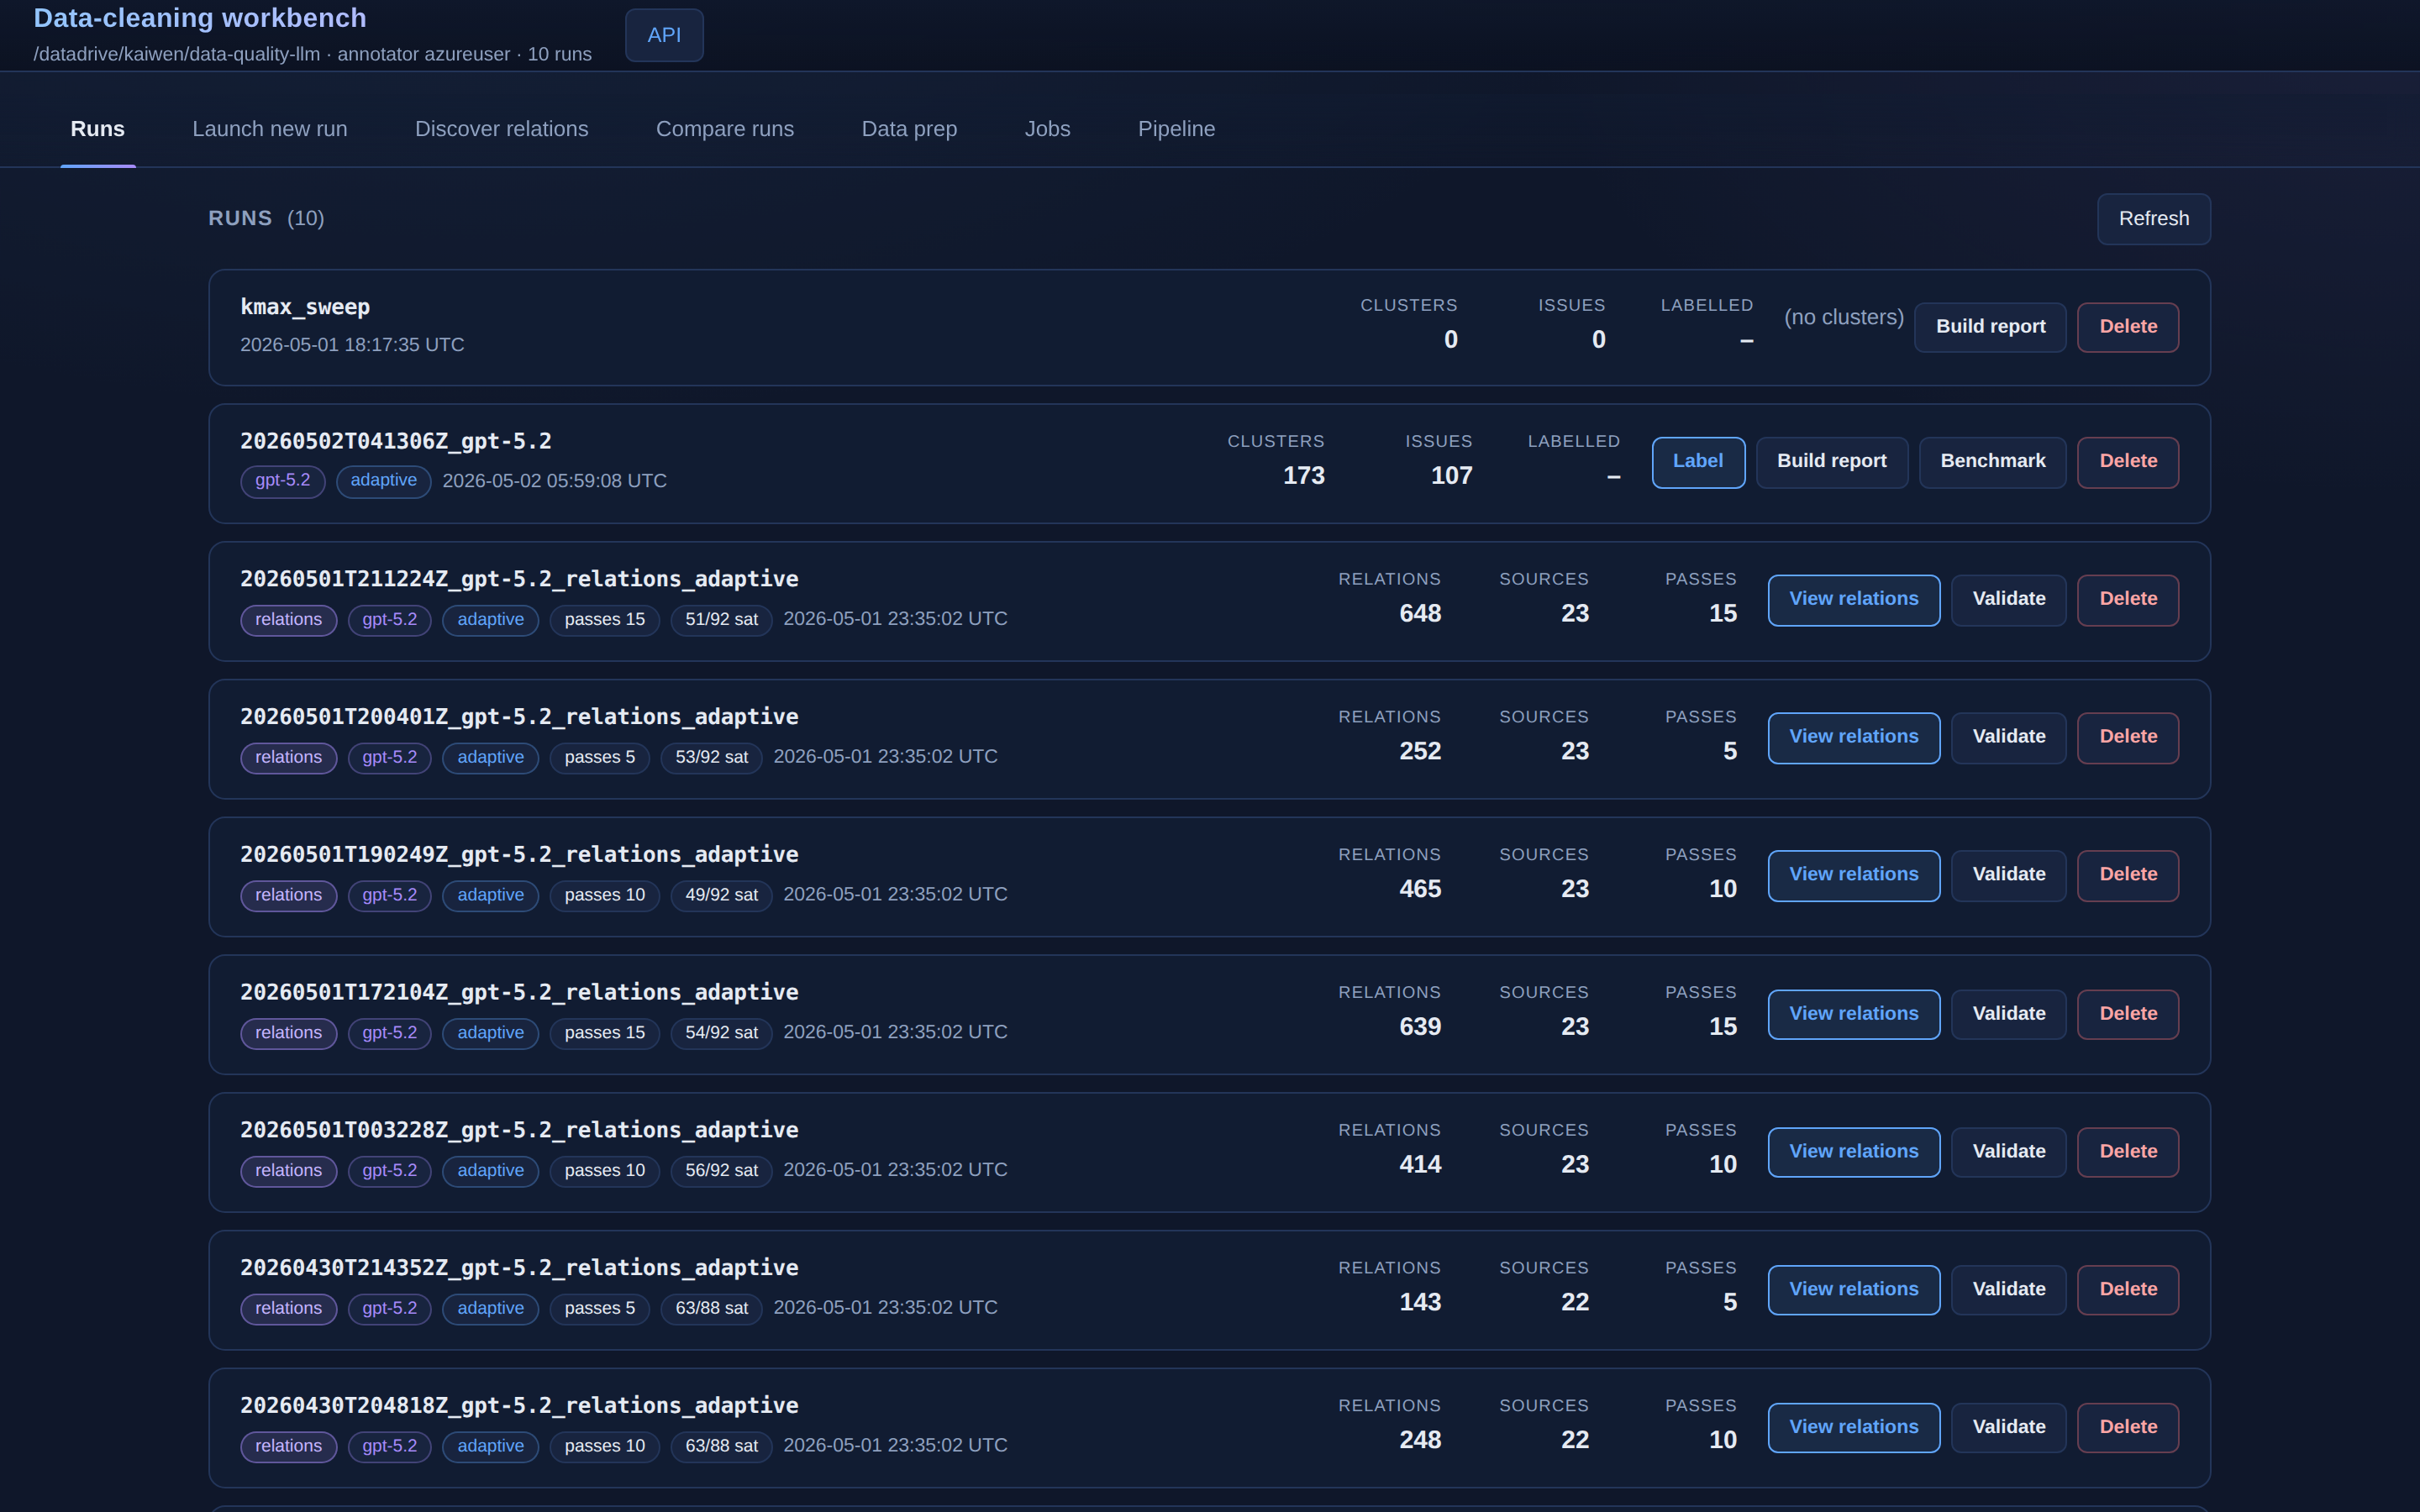
\includegraphics[width=0.86\linewidth]{screenshot_runs_dashboard.png}
\caption{Runs dashboard --- launch, browse, and compare runs.}
\label{fig:dashboard}
\end{figure}

\begin{figure}[h]
\centering
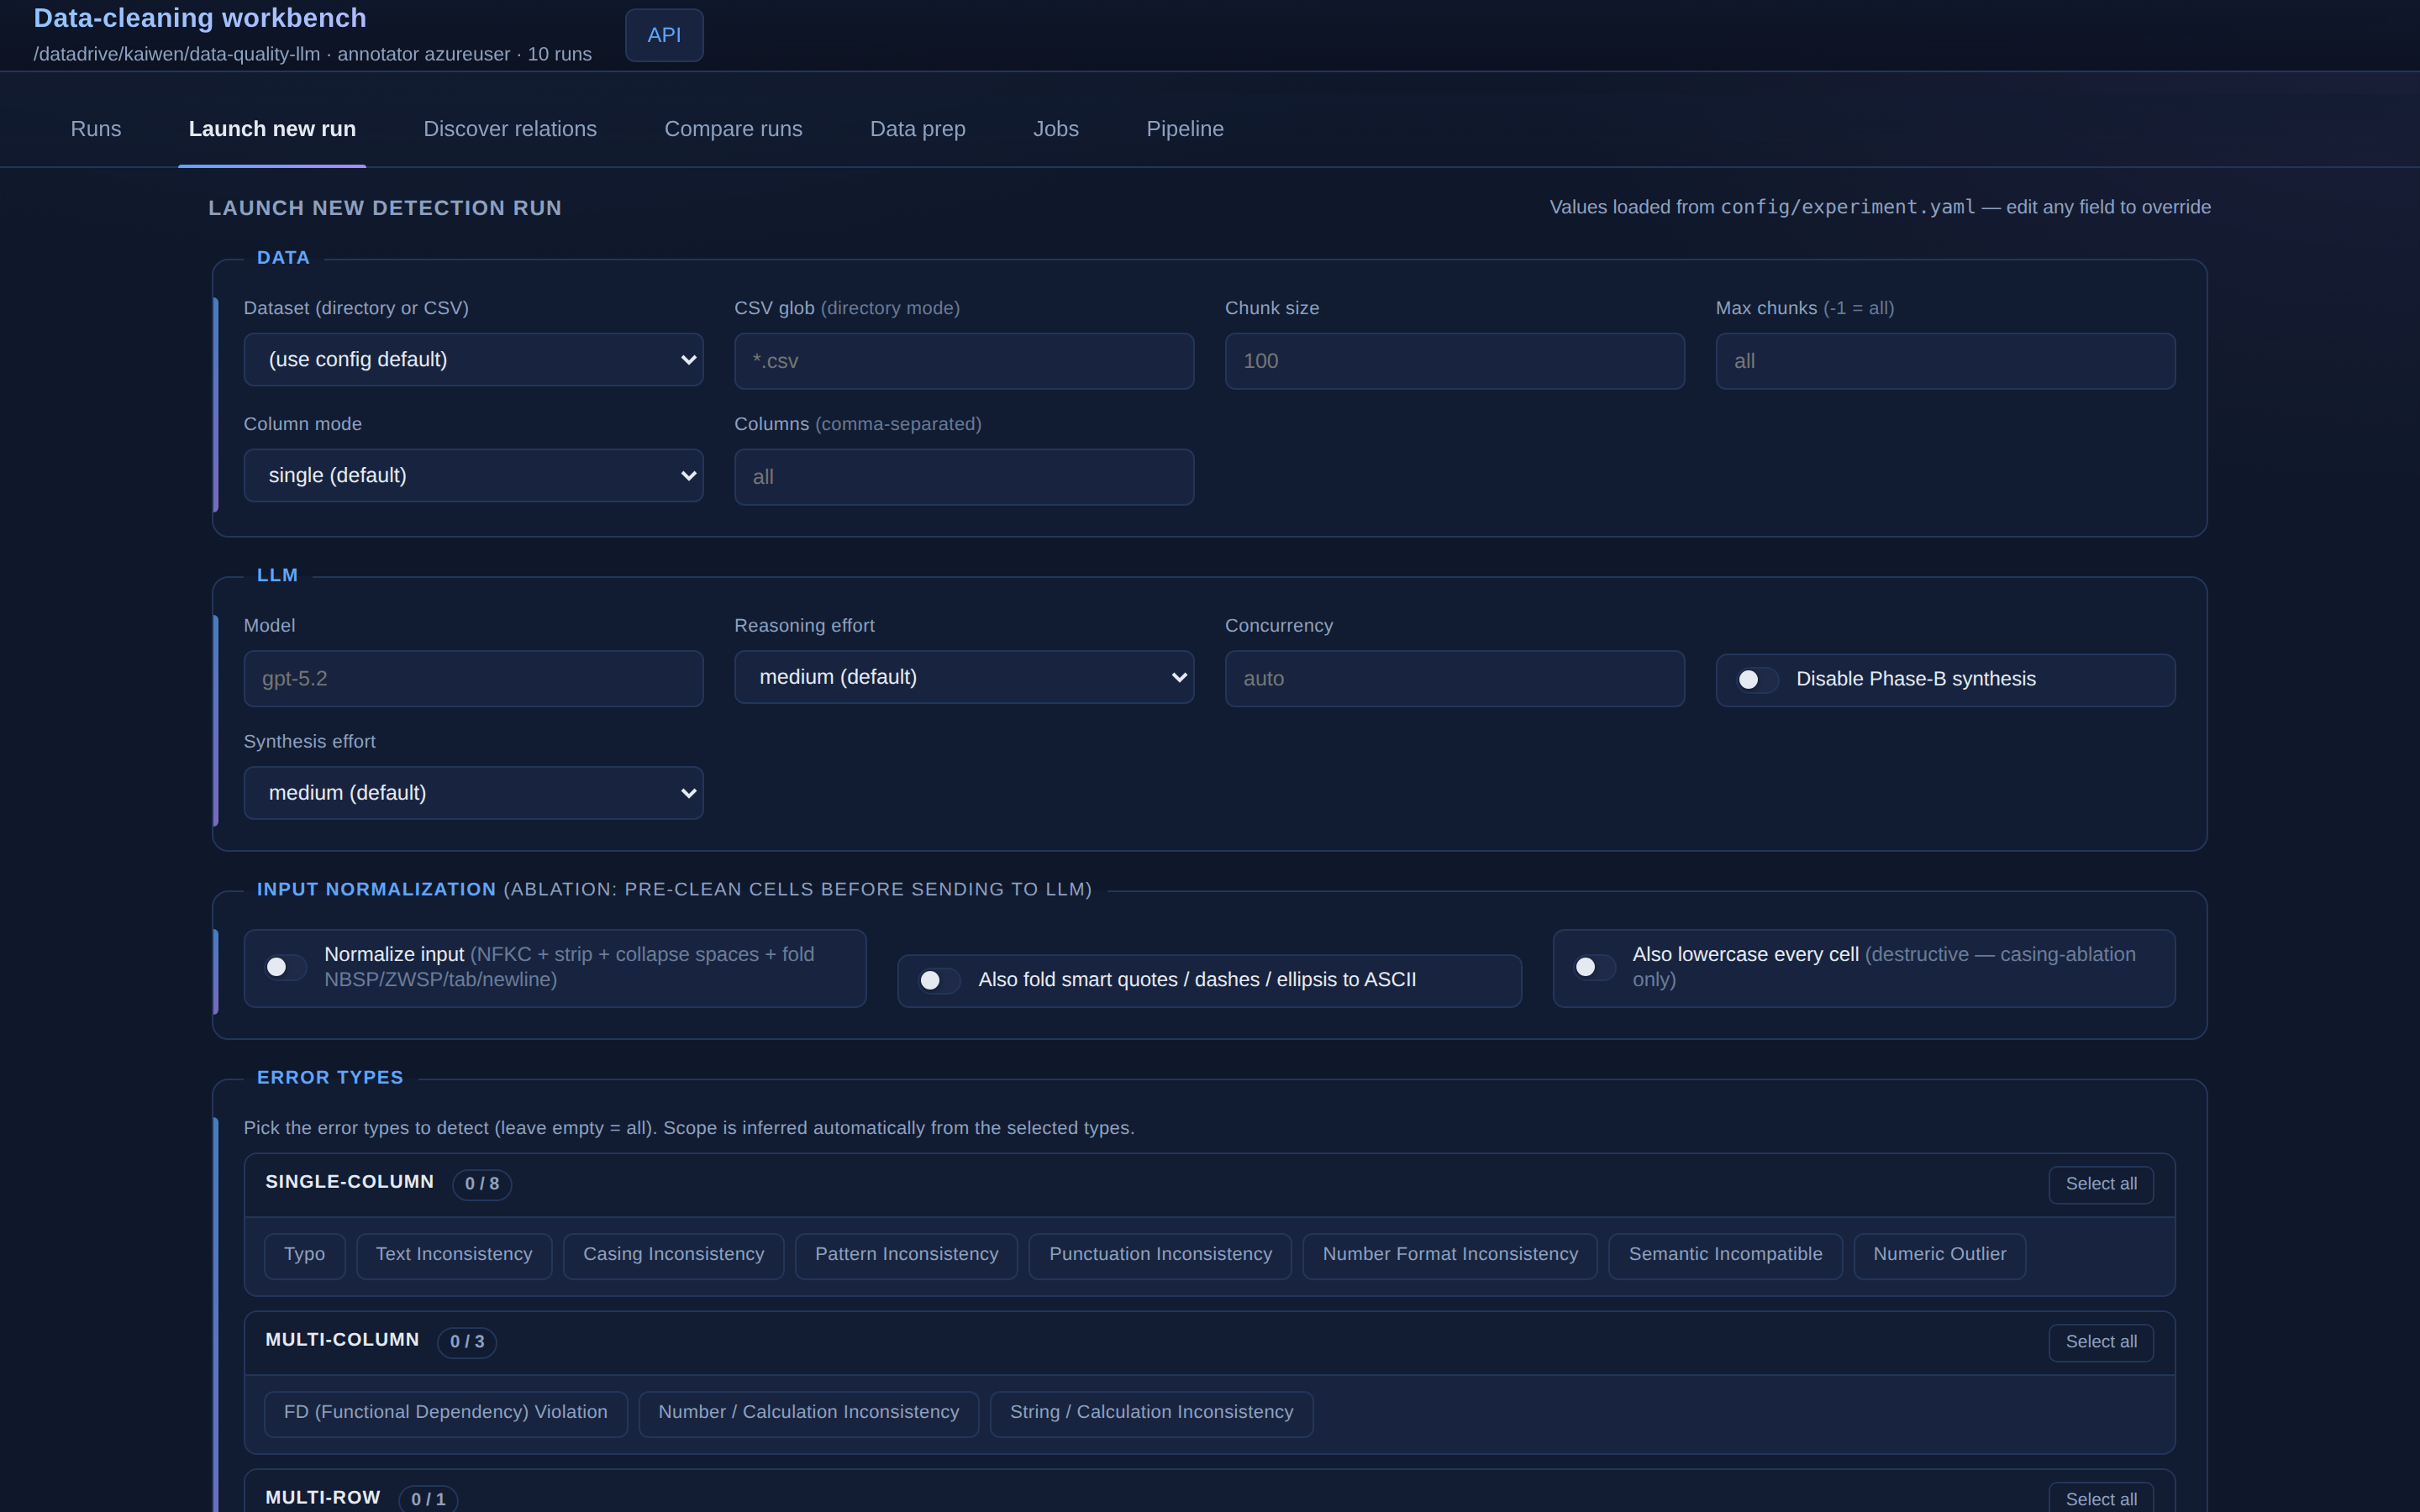
\includegraphics[width=0.86\linewidth]{screenshot_launch_form.png}
\caption{Launch-new-run form.}
\label{fig:launch}
\end{figure}

\begin{figure}[h]
\centering
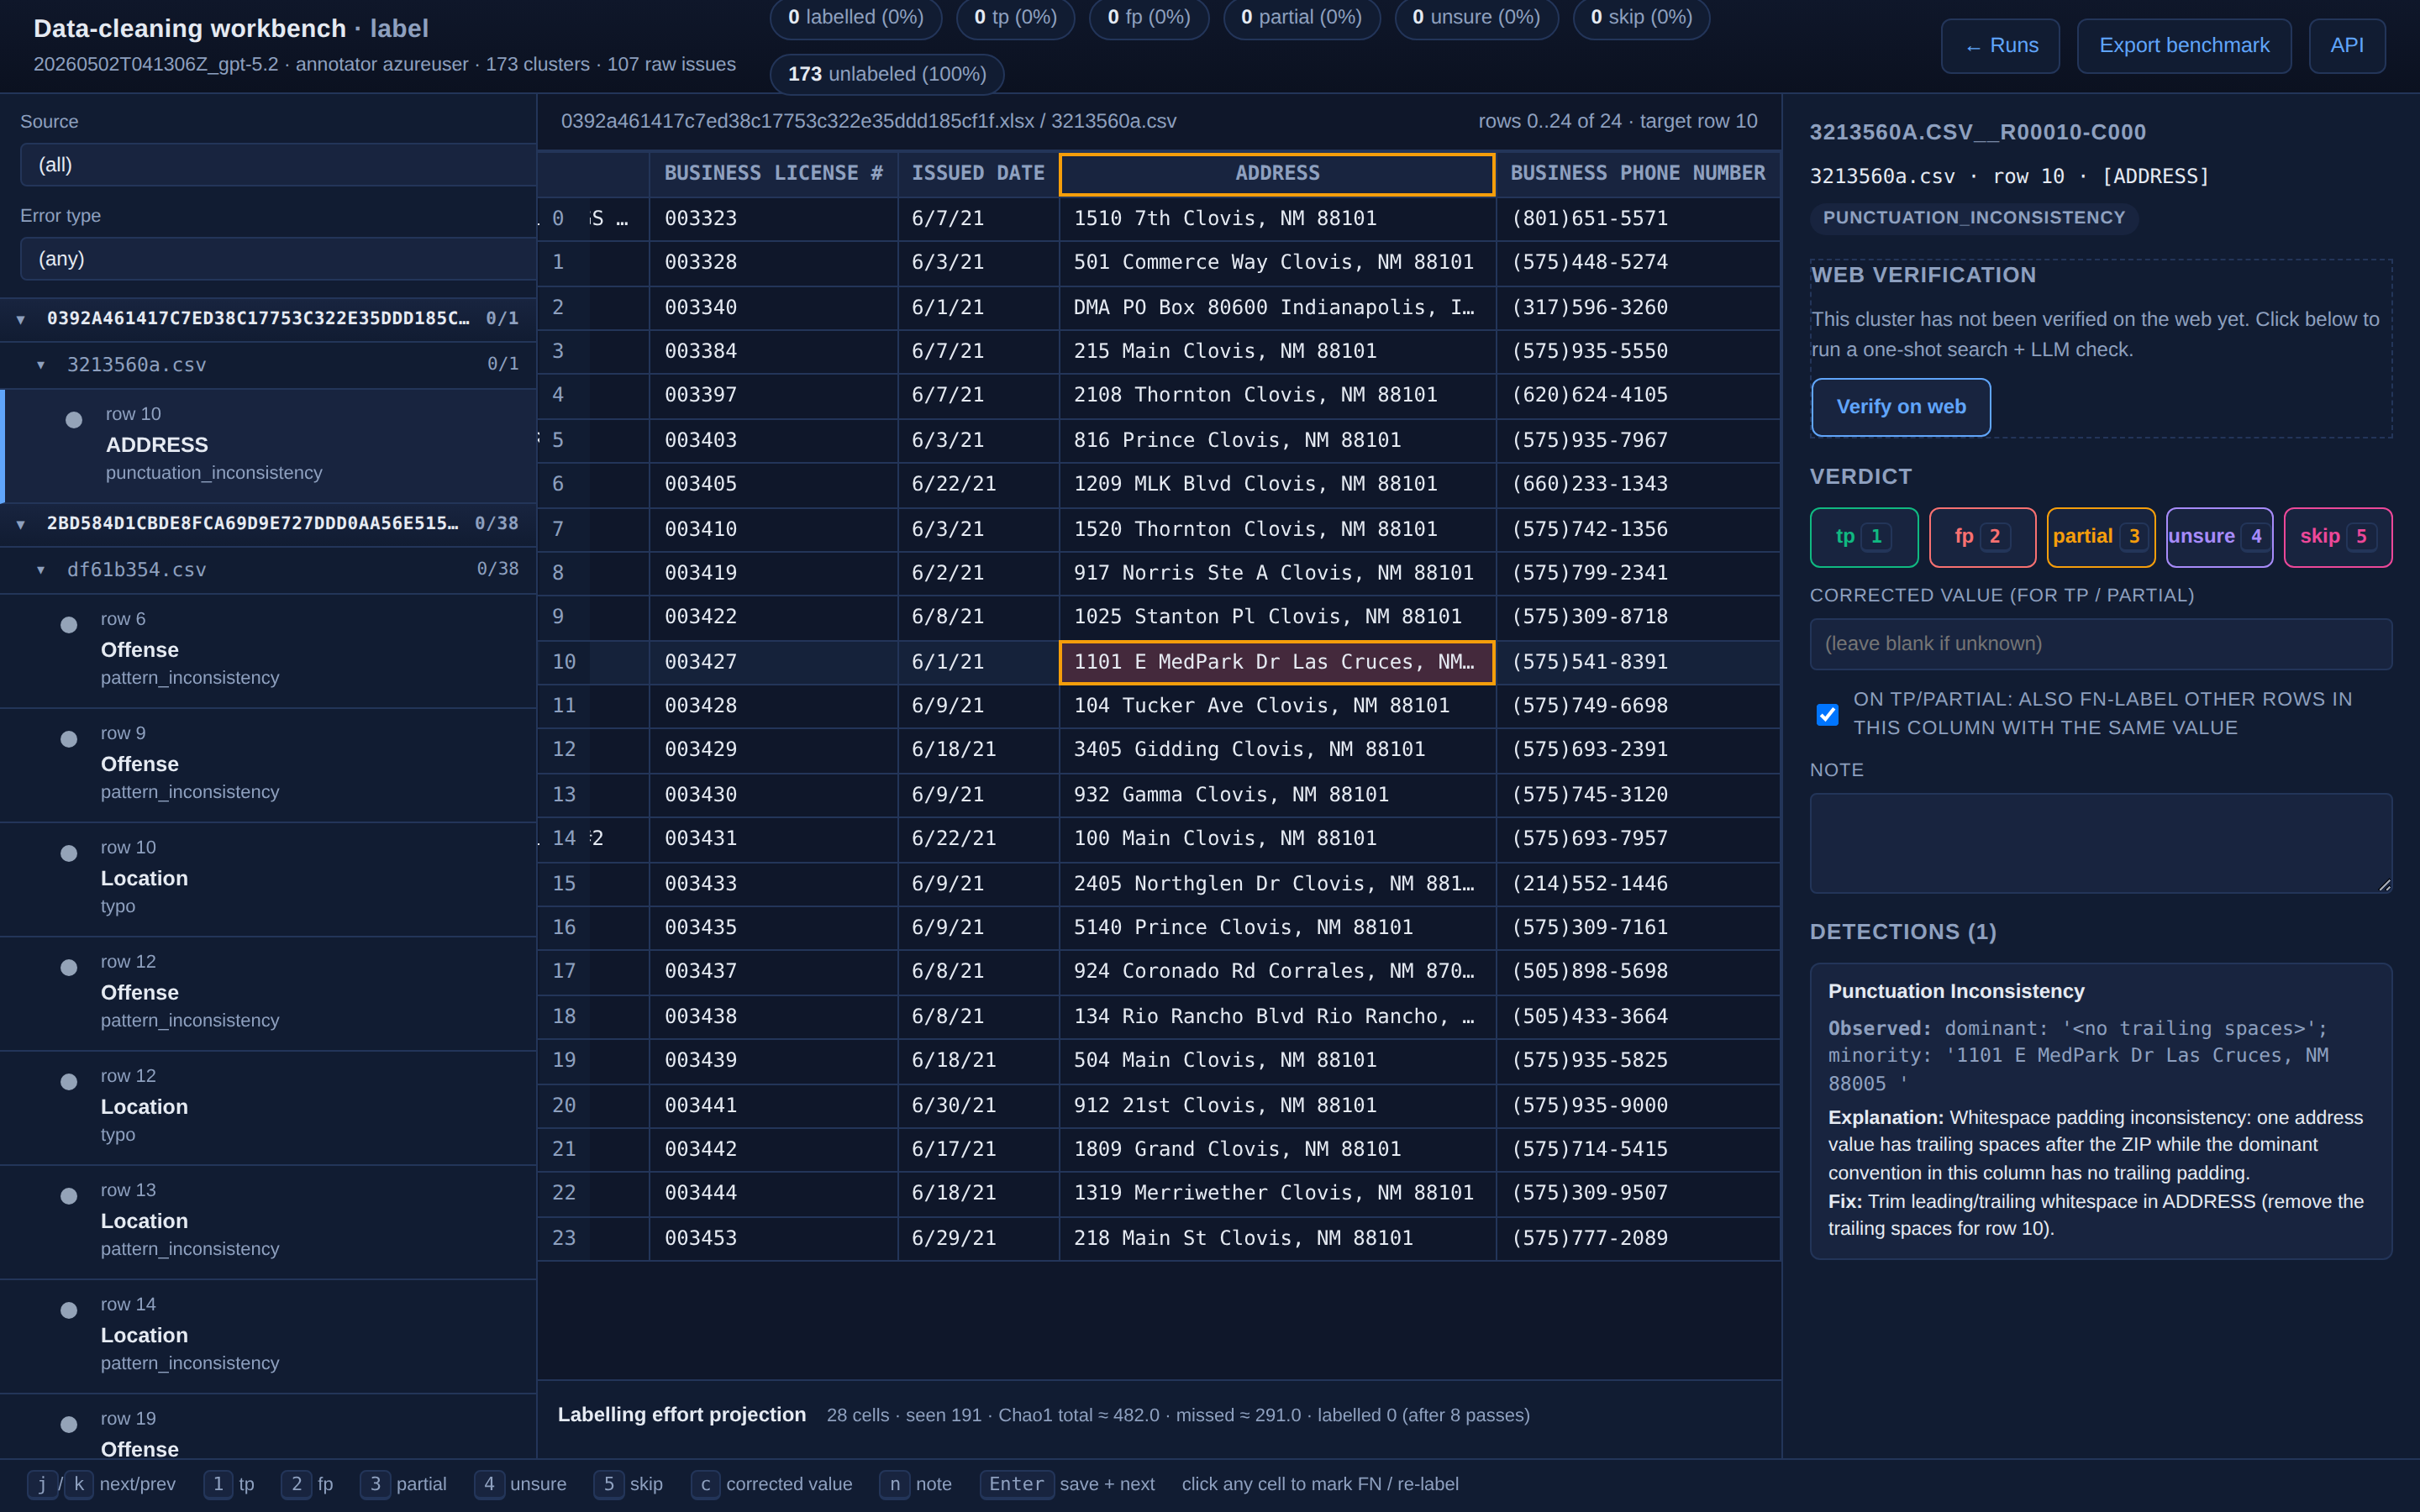
\includegraphics[width=0.86\linewidth]{screenshot_labeling_view.png}
\caption{Labelling view: flagged cells in source context.}
\label{fig:labeling}
\end{figure}

\begin{figure}[h]
\centering
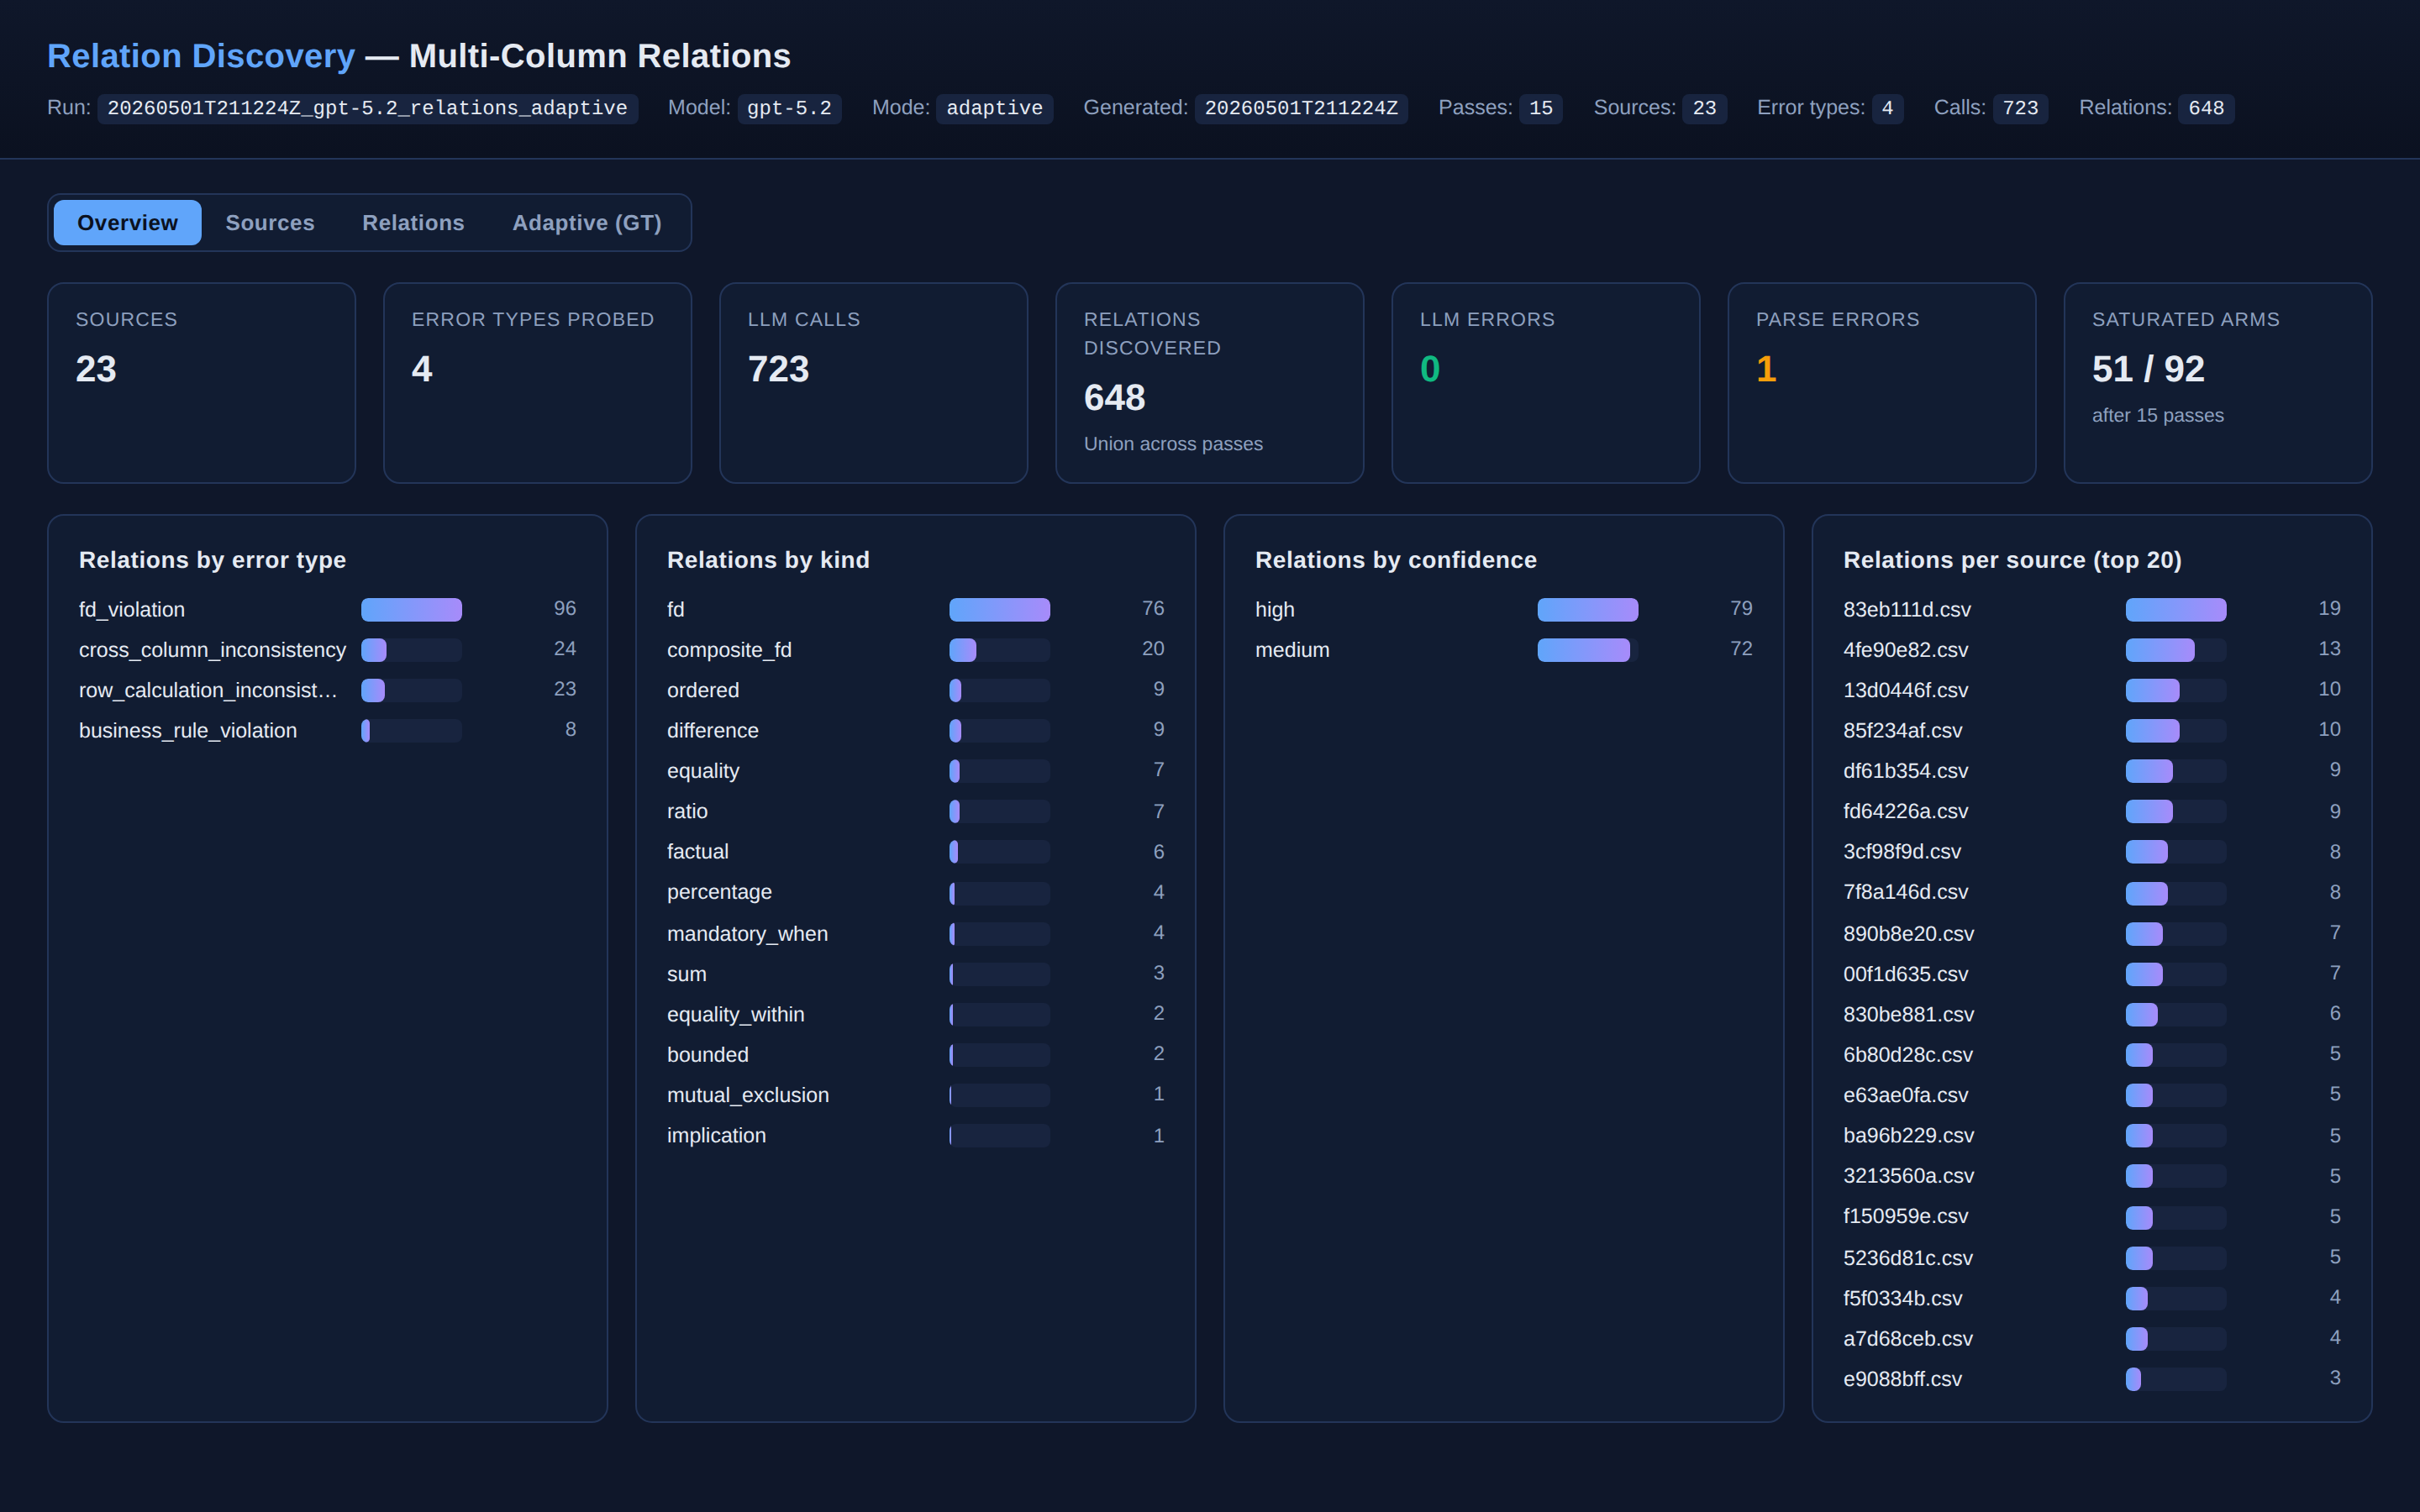
\includegraphics[width=0.86\linewidth]{screenshot_html_report.png}
\caption{Self-contained HTML report.}
\label{fig:report}
\end{figure}

\end{document}
